% Options for packages loaded elsewhere
\PassOptionsToPackage{unicode}{hyperref}
\PassOptionsToPackage{hyphens}{url}
\PassOptionsToPackage{dvipsnames,svgnames,x11names}{xcolor}
%
\documentclass[
  letterpaper,
  DIV=11,
  numbers=noendperiod]{scrreprt}

\usepackage{amsmath,amssymb}
\usepackage{lmodern}
\usepackage{iftex}
\ifPDFTeX
  \usepackage[T1]{fontenc}
  \usepackage[utf8]{inputenc}
  \usepackage{textcomp} % provide euro and other symbols
\else % if luatex or xetex
  \usepackage{unicode-math}
  \defaultfontfeatures{Scale=MatchLowercase}
  \defaultfontfeatures[\rmfamily]{Ligatures=TeX,Scale=1}
\fi
% Use upquote if available, for straight quotes in verbatim environments
\IfFileExists{upquote.sty}{\usepackage{upquote}}{}
\IfFileExists{microtype.sty}{% use microtype if available
  \usepackage[]{microtype}
  \UseMicrotypeSet[protrusion]{basicmath} % disable protrusion for tt fonts
}{}
\makeatletter
\@ifundefined{KOMAClassName}{% if non-KOMA class
  \IfFileExists{parskip.sty}{%
    \usepackage{parskip}
  }{% else
    \setlength{\parindent}{0pt}
    \setlength{\parskip}{6pt plus 2pt minus 1pt}}
}{% if KOMA class
  \KOMAoptions{parskip=half}}
\makeatother
\usepackage{xcolor}
\setlength{\emergencystretch}{3em} % prevent overfull lines
\setcounter{secnumdepth}{5}
% Make \paragraph and \subparagraph free-standing
\ifx\paragraph\undefined\else
  \let\oldparagraph\paragraph
  \renewcommand{\paragraph}[1]{\oldparagraph{#1}\mbox{}}
\fi
\ifx\subparagraph\undefined\else
  \let\oldsubparagraph\subparagraph
  \renewcommand{\subparagraph}[1]{\oldsubparagraph{#1}\mbox{}}
\fi

\usepackage{color}
\usepackage{fancyvrb}
\newcommand{\VerbBar}{|}
\newcommand{\VERB}{\Verb[commandchars=\\\{\}]}
\DefineVerbatimEnvironment{Highlighting}{Verbatim}{commandchars=\\\{\}}
% Add ',fontsize=\small' for more characters per line
\usepackage{framed}
\definecolor{shadecolor}{RGB}{241,243,245}
\newenvironment{Shaded}{\begin{snugshade}}{\end{snugshade}}
\newcommand{\AlertTok}[1]{\textcolor[rgb]{0.68,0.00,0.00}{#1}}
\newcommand{\AnnotationTok}[1]{\textcolor[rgb]{0.37,0.37,0.37}{#1}}
\newcommand{\AttributeTok}[1]{\textcolor[rgb]{0.40,0.45,0.13}{#1}}
\newcommand{\BaseNTok}[1]{\textcolor[rgb]{0.68,0.00,0.00}{#1}}
\newcommand{\BuiltInTok}[1]{\textcolor[rgb]{0.00,0.23,0.31}{#1}}
\newcommand{\CharTok}[1]{\textcolor[rgb]{0.13,0.47,0.30}{#1}}
\newcommand{\CommentTok}[1]{\textcolor[rgb]{0.37,0.37,0.37}{#1}}
\newcommand{\CommentVarTok}[1]{\textcolor[rgb]{0.37,0.37,0.37}{\textit{#1}}}
\newcommand{\ConstantTok}[1]{\textcolor[rgb]{0.56,0.35,0.01}{#1}}
\newcommand{\ControlFlowTok}[1]{\textcolor[rgb]{0.00,0.23,0.31}{#1}}
\newcommand{\DataTypeTok}[1]{\textcolor[rgb]{0.68,0.00,0.00}{#1}}
\newcommand{\DecValTok}[1]{\textcolor[rgb]{0.68,0.00,0.00}{#1}}
\newcommand{\DocumentationTok}[1]{\textcolor[rgb]{0.37,0.37,0.37}{\textit{#1}}}
\newcommand{\ErrorTok}[1]{\textcolor[rgb]{0.68,0.00,0.00}{#1}}
\newcommand{\ExtensionTok}[1]{\textcolor[rgb]{0.00,0.23,0.31}{#1}}
\newcommand{\FloatTok}[1]{\textcolor[rgb]{0.68,0.00,0.00}{#1}}
\newcommand{\FunctionTok}[1]{\textcolor[rgb]{0.28,0.35,0.67}{#1}}
\newcommand{\ImportTok}[1]{\textcolor[rgb]{0.00,0.46,0.62}{#1}}
\newcommand{\InformationTok}[1]{\textcolor[rgb]{0.37,0.37,0.37}{#1}}
\newcommand{\KeywordTok}[1]{\textcolor[rgb]{0.00,0.23,0.31}{#1}}
\newcommand{\NormalTok}[1]{\textcolor[rgb]{0.00,0.23,0.31}{#1}}
\newcommand{\OperatorTok}[1]{\textcolor[rgb]{0.37,0.37,0.37}{#1}}
\newcommand{\OtherTok}[1]{\textcolor[rgb]{0.00,0.23,0.31}{#1}}
\newcommand{\PreprocessorTok}[1]{\textcolor[rgb]{0.68,0.00,0.00}{#1}}
\newcommand{\RegionMarkerTok}[1]{\textcolor[rgb]{0.00,0.23,0.31}{#1}}
\newcommand{\SpecialCharTok}[1]{\textcolor[rgb]{0.37,0.37,0.37}{#1}}
\newcommand{\SpecialStringTok}[1]{\textcolor[rgb]{0.13,0.47,0.30}{#1}}
\newcommand{\StringTok}[1]{\textcolor[rgb]{0.13,0.47,0.30}{#1}}
\newcommand{\VariableTok}[1]{\textcolor[rgb]{0.07,0.07,0.07}{#1}}
\newcommand{\VerbatimStringTok}[1]{\textcolor[rgb]{0.13,0.47,0.30}{#1}}
\newcommand{\WarningTok}[1]{\textcolor[rgb]{0.37,0.37,0.37}{\textit{#1}}}

\providecommand{\tightlist}{%
  \setlength{\itemsep}{0pt}\setlength{\parskip}{0pt}}\usepackage{longtable,booktabs,array}
\usepackage{calc} % for calculating minipage widths
% Correct order of tables after \paragraph or \subparagraph
\usepackage{etoolbox}
\makeatletter
\patchcmd\longtable{\par}{\if@noskipsec\mbox{}\fi\par}{}{}
\makeatother
% Allow footnotes in longtable head/foot
\IfFileExists{footnotehyper.sty}{\usepackage{footnotehyper}}{\usepackage{footnote}}
\makesavenoteenv{longtable}
\usepackage{graphicx}
\makeatletter
\def\maxwidth{\ifdim\Gin@nat@width>\linewidth\linewidth\else\Gin@nat@width\fi}
\def\maxheight{\ifdim\Gin@nat@height>\textheight\textheight\else\Gin@nat@height\fi}
\makeatother
% Scale images if necessary, so that they will not overflow the page
% margins by default, and it is still possible to overwrite the defaults
% using explicit options in \includegraphics[width, height, ...]{}
\setkeys{Gin}{width=\maxwidth,height=\maxheight,keepaspectratio}
% Set default figure placement to htbp
\makeatletter
\def\fps@figure{htbp}
\makeatother

<script src="site_libs/font-awesome-5.13.0/js/script.js"></script>
\KOMAoption{captions}{tableheading}
\makeatletter
\makeatother
\makeatletter
\@ifpackageloaded{bookmark}{}{\usepackage{bookmark}}
\makeatother
\makeatletter
\@ifpackageloaded{caption}{}{\usepackage{caption}}
\AtBeginDocument{%
\ifdefined\contentsname
  \renewcommand*\contentsname{Table of contents}
\else
  \newcommand\contentsname{Table of contents}
\fi
\ifdefined\listfigurename
  \renewcommand*\listfigurename{List of Figures}
\else
  \newcommand\listfigurename{List of Figures}
\fi
\ifdefined\listtablename
  \renewcommand*\listtablename{List of Tables}
\else
  \newcommand\listtablename{List of Tables}
\fi
\ifdefined\figurename
  \renewcommand*\figurename{Figure}
\else
  \newcommand\figurename{Figure}
\fi
\ifdefined\tablename
  \renewcommand*\tablename{Table}
\else
  \newcommand\tablename{Table}
\fi
}
\@ifpackageloaded{float}{}{\usepackage{float}}
\floatstyle{ruled}
\@ifundefined{c@chapter}{\newfloat{codelisting}{h}{lop}}{\newfloat{codelisting}{h}{lop}[chapter]}
\floatname{codelisting}{Listing}
\newcommand*\listoflistings{\listof{codelisting}{List of Listings}}
\makeatother
\makeatletter
\@ifpackageloaded{caption}{}{\usepackage{caption}}
\@ifpackageloaded{subcaption}{}{\usepackage{subcaption}}
\makeatother
\makeatletter
\@ifpackageloaded{tcolorbox}{}{\usepackage[many]{tcolorbox}}
\makeatother
\makeatletter
\@ifundefined{shadecolor}{\definecolor{shadecolor}{rgb}{.97, .97, .97}}
\makeatother
\makeatletter
\makeatother
\ifLuaTeX
  \usepackage{selnolig}  % disable illegal ligatures
\fi
\IfFileExists{bookmark.sty}{\usepackage{bookmark}}{\usepackage{hyperref}}
\IfFileExists{xurl.sty}{\usepackage{xurl}}{} % add URL line breaks if available
\urlstyle{same} % disable monospaced font for URLs
\hypersetup{
  pdftitle={Models for Multi-State Survival Data: Rates, Risks, and Pseudo-Values},
  pdfauthor={Per Kragh Andersen and Henrik Ravn},
  colorlinks=true,
  linkcolor={blue},
  filecolor={Maroon},
  citecolor={Blue},
  urlcolor={Blue},
  pdfcreator={LaTeX via pandoc}}

\title{Models for Multi-State Survival Data: Rates, Risks, and
Pseudo-Values}
\author{Per Kragh Andersen and Henrik Ravn}
\date{}

\begin{document}
\maketitle
\ifdefined\Shaded\renewenvironment{Shaded}{\begin{tcolorbox}[frame hidden, borderline west={3pt}{0pt}{shadecolor}, interior hidden, breakable, enhanced, boxrule=0pt, sharp corners]}{\end{tcolorbox}}\fi

\renewcommand*\contentsname{Table of contents}
{
\hypersetup{linkcolor=}
\setcounter{tocdepth}{2}
\tableofcontents
}
\bookmarksetup{startatroot}

\hypertarget{preface}{%
\chapter*{Preface}\label{preface}}
\addcontentsline{toc}{chapter}{Preface}

\markboth{Preface}{Preface}

This is the companion website to the book \textbf{Models for Multi-State
Survival Data: Rates, Risks, and Pseudo-Values}, published by Chapman \&
Hall (link).

R and SAS code for all the an alyses presented in the book is available,
except for analyses on the xxx data. The plots in the book are created
using R and available as presented in the book and accompanied with a
crude SAS version.

Solutions to the book exercises are available at the end of the
chapters.

\hypertarget{acknowledgements}{%
\section*{Acknowledgements}\label{acknowledgements}}
\addcontentsline{toc}{section}{Acknowledgements}

\markright{Acknowledgements}

Julie and Eva

\bookmarksetup{startatroot}

\hypertarget{introduction-with-data-sets}{%
\chapter{Introduction with data
sets}\label{introduction-with-data-sets}}

In the book, a series of examples of event history data are used to
illustrate different methods, models and approaches. Here most of the
data sets are available for download together with a description of the
variables.

You can download \textbf{all} available data sets in one zip file or the
individual data sets from following sections.

\hypertarget{the-pbc3-trial-in-liver-cirrhosis}{%
\section{The PBC3 trial in liver
cirrhosis}\label{the-pbc3-trial-in-liver-cirrhosis}}

PBC3 was a multi-center randomized clinical trial conducted in six
European hospitals (Lombard et al., 1993). Between January 1983 and
January 1989, 349 patients with the liver disease primary biliary
cirrhosis (PBC) were randomized to treatment with either Cyclosporin A
(CyA, 176 patients) or placebo (173 patients).

\hypertarget{the-guinea-bissau-childhood-vaccination-study}{%
\section{The Guinea-Bissau childhood vaccination
study}\label{the-guinea-bissau-childhood-vaccination-study}}

A longitudinal study of children was initiated in 1990 in five regions
of Guinea-Bissau, West Africa.

\begin{longtable}[]{@{}ll@{}}
\toprule()
Variable name & Description and labels \\
\midrule()
\endhead
id & id variable for the child \\
fuptime & follow-up time in days \\
dead & status at fuptime (0 alive, 1 dead) \\
bcg & bcg vaccination status at initial visit (1=yes, 2=no) \\
dtp & dtp vaccination status at initial visit (1=yes, 2=no) \\
age & age in days at initial visit \\
agem & age in months at initial visit \\
\bottomrule()
\end{longtable}

\hypertarget{testis-cancer-incidence-and-maternal-parity}{%
\section{Testis cancer incidence and maternal
parity}\label{testis-cancer-incidence-and-maternal-parity}}

\hypertarget{prova-trial-in-liver-cirrhosis}{%
\section{PROVA trial in liver
cirrhosis}\label{prova-trial-in-liver-cirrhosis}}

\hypertarget{recurrent-episodes-in-affective-disorders}{%
\section{Recurrent episodes in affective
disorders}\label{recurrent-episodes-in-affective-disorders}}

\hypertarget{leader-trial-in-type-2-diabetes}{%
\section{LEADER trial in Type 2
Diabetes}\label{leader-trial-in-type-2-diabetes}}

\hypertarget{the-copenhagen-holter-study}{%
\section{The Copenhagen Holter
study}\label{the-copenhagen-holter-study}}

\bookmarksetup{startatroot}

\hypertarget{intuition-for-models-for-intensities}{%
\chapter{Intuition for models for
intensities}\label{intuition-for-models-for-intensities}}

\begin{verbatim}
Loading required package: survival
\end{verbatim}

\begin{verbatim}
Warning: package 'survival' was built under R version 4.2.2
\end{verbatim}

\begin{verbatim}
Loading required package: tidyverse
\end{verbatim}

\begin{verbatim}
Warning: package 'tidyverse' was built under R version 4.2.2
\end{verbatim}

\begin{verbatim}
-- Attaching packages ------------------- tidyverse 1.3.2 --
\end{verbatim}

\begin{verbatim}
v ggplot2 3.3.6     v purrr   0.3.4
v tibble  3.1.7     v dplyr   1.0.9
v tidyr   1.2.0     v stringr 1.4.0
v readr   2.1.2     v forcats 0.5.1
-- Conflicts ---------------------- tidyverse_conflicts() --
x dplyr::filter() masks stats::filter()
x dplyr::lag()    masks stats::lag()
Loading required package: timereg

Loading required package: gridExtra


Attaching package: 'gridExtra'


The following object is masked from 'package:dplyr':

    combine
\end{verbatim}

\[\alpha(t)=\alpha_0(t)\exp(\beta Z)\]

\hypertarget{fig2-2}{%
\section*{Figure 2.2}\label{fig2-2}}
\addcontentsline{toc}{section}{Figure 2.2}

\markright{Figure 2.2}

\begin{Shaded}
\begin{Highlighting}[]
\NormalTok{pbc3}\OtherTok{\textless{}{-}}\FunctionTok{readRDS}\NormalTok{(}\StringTok{"data/pbc3.rds"}\NormalTok{)}
\NormalTok{nafit }\OtherTok{\textless{}{-}} \FunctionTok{survfit}\NormalTok{(}\FunctionTok{Surv}\NormalTok{(followup, status }\SpecialCharTok{!=} \DecValTok{0}\NormalTok{) }\SpecialCharTok{\textasciitilde{}}\NormalTok{ tment, }\AttributeTok{data =}\NormalTok{ pbc3)}
\NormalTok{nadata }\OtherTok{\textless{}{-}} \FunctionTok{data.frame}\NormalTok{(}\AttributeTok{cumhaz =}\NormalTok{ nafit}\SpecialCharTok{$}\NormalTok{cumhaz, }
                     \AttributeTok{cumhaz\_se =}\NormalTok{ nafit}\SpecialCharTok{$}\NormalTok{std.err, }
                     \AttributeTok{time =}\NormalTok{ nafit}\SpecialCharTok{$}\NormalTok{time, }
                     \AttributeTok{tment =} \FunctionTok{c}\NormalTok{(}\FunctionTok{rep}\NormalTok{(}\FunctionTok{names}\NormalTok{(nafit}\SpecialCharTok{$}\NormalTok{strata)[}\DecValTok{1}\NormalTok{], nafit}\SpecialCharTok{$}\NormalTok{strata[}\DecValTok{1}\NormalTok{]), }
                               \FunctionTok{rep}\NormalTok{(}\FunctionTok{names}\NormalTok{(nafit}\SpecialCharTok{$}\NormalTok{strata)[}\DecValTok{2}\NormalTok{], nafit}\SpecialCharTok{$}\NormalTok{strata[}\DecValTok{2}\NormalTok{])))}

\CommentTok{\# Create Figure 2.2}
\FunctionTok{ggplot}\NormalTok{(}\FunctionTok{aes}\NormalTok{(}\AttributeTok{x =}\NormalTok{ time, }\AttributeTok{y =}\NormalTok{ cumhaz, }\AttributeTok{linetype =}\NormalTok{ tment), }\AttributeTok{data =}\NormalTok{ nadata) }\SpecialCharTok{+} 
          \FunctionTok{geom\_step}\NormalTok{(}\AttributeTok{size =} \DecValTok{1}\NormalTok{) }\SpecialCharTok{+} 
          \FunctionTok{scale\_linetype\_discrete}\NormalTok{(}\StringTok{"Treatment"}\NormalTok{, }\AttributeTok{labels =} \FunctionTok{c}\NormalTok{(}\StringTok{"Placebo"}\NormalTok{, }\StringTok{"CyA"}\NormalTok{)) }\SpecialCharTok{+} 
          \FunctionTok{xlab}\NormalTok{(}\StringTok{"Time since randomization (years)"}\NormalTok{) }\SpecialCharTok{+} 
          \FunctionTok{ylab}\NormalTok{(}\StringTok{"Cumulative hazard"}\NormalTok{) }\SpecialCharTok{+} 
          \FunctionTok{scale\_x\_continuous}\NormalTok{(}\AttributeTok{expand =} \FunctionTok{expansion}\NormalTok{(}\AttributeTok{mult =} \FunctionTok{c}\NormalTok{(}\FloatTok{0.005}\NormalTok{, }\FloatTok{0.05}\NormalTok{)), ) }\SpecialCharTok{+} 
          \FunctionTok{scale\_y\_continuous}\NormalTok{(}\AttributeTok{expand =} \FunctionTok{expansion}\NormalTok{(}\AttributeTok{mult =} \FunctionTok{c}\NormalTok{(}\FloatTok{0.005}\NormalTok{, }\FloatTok{0.05}\NormalTok{))) }\SpecialCharTok{+}
\NormalTok{          theme\_general}
\end{Highlighting}
\end{Shaded}

\begin{figure}[H]

{\centering 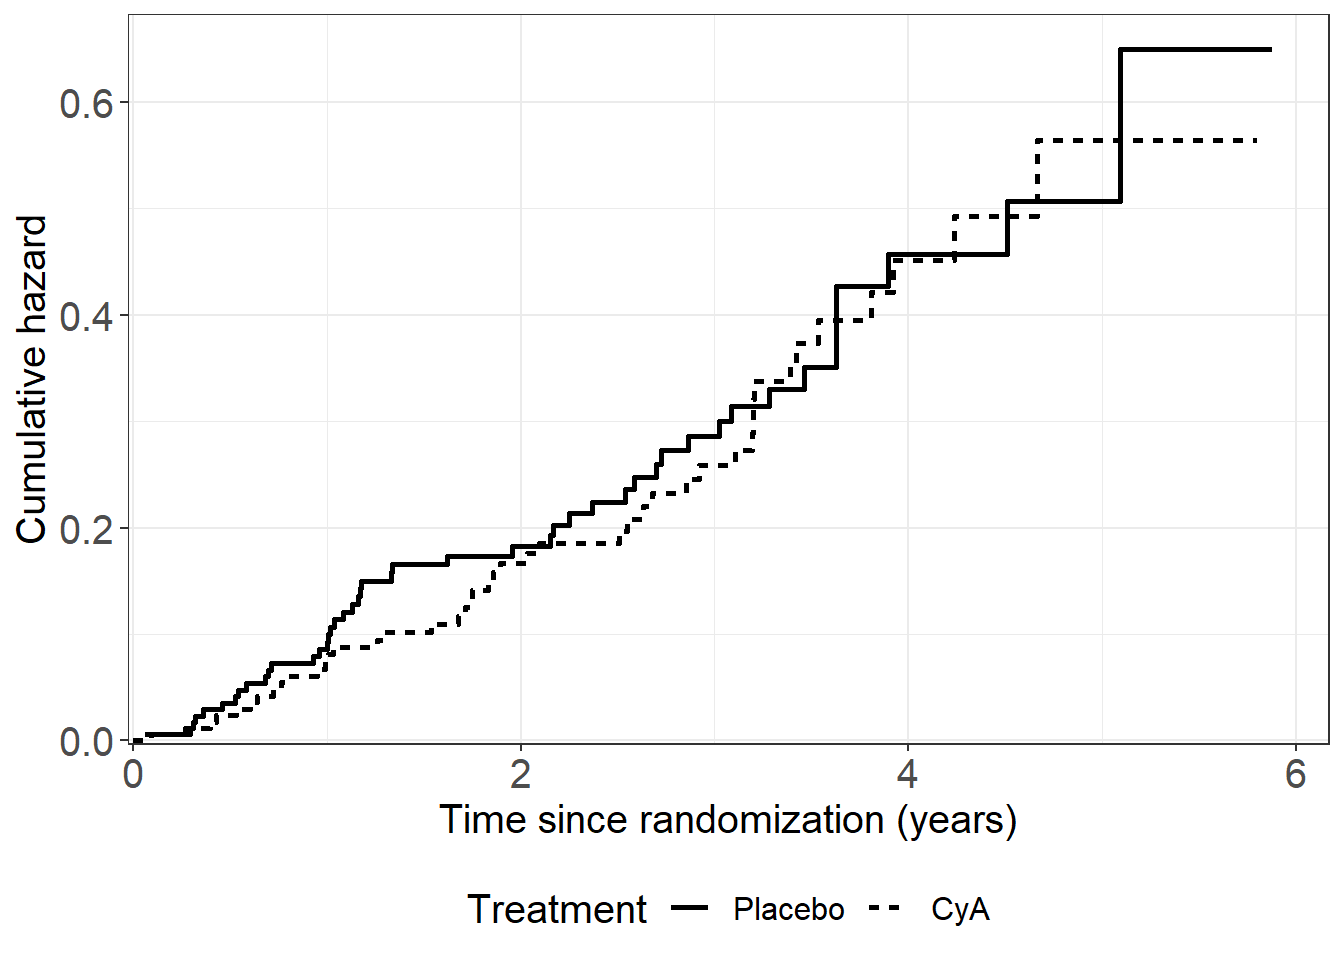
\includegraphics{./Ch2_files/figure-pdf/unnamed-chunk-2-1.pdf}

}

\end{figure}

\hypertarget{fig2-3}{%
\section*{Figure 2.3}\label{fig2-3}}
\addcontentsline{toc}{section}{Figure 2.3}

\markright{Figure 2.3}

\begin{Shaded}
\begin{Highlighting}[]
\NormalTok{rateCyA }\OtherTok{\textless{}{-}} \FunctionTok{c}\NormalTok{(}\FloatTok{8.1}\NormalTok{,}\FloatTok{13.1}\NormalTok{,}\FloatTok{9.6}\NormalTok{)}
\NormalTok{ratePbo }\OtherTok{\textless{}{-}} \FunctionTok{c}\NormalTok{(}\FloatTok{9.4}\NormalTok{,}\FloatTok{12.5}\NormalTok{,}\FloatTok{8.5}\NormalTok{)}
\NormalTok{pcwtime }\OtherTok{\textless{}{-}} \FunctionTok{c}\NormalTok{(}\DecValTok{0}\NormalTok{,}\DecValTok{2}\NormalTok{,}\DecValTok{4}\NormalTok{,}\DecValTok{5}\NormalTok{)}

\CommentTok{\# Collect data}
\NormalTok{plotdata }\OtherTok{\textless{}{-}} \FunctionTok{data.frame}\NormalTok{(}\AttributeTok{rates =} \FunctionTok{c}\NormalTok{(rateCyA, ratePbo),}
                       \AttributeTok{tment =} \FunctionTok{c}\NormalTok{(}\FunctionTok{rep}\NormalTok{(}\StringTok{"CyA"}\NormalTok{, }\FunctionTok{length}\NormalTok{(rateCyA)), }\FunctionTok{rep}\NormalTok{(}\StringTok{"Placebo"}\NormalTok{, }\FunctionTok{length}\NormalTok{(ratePbo))),}
                       \AttributeTok{times\_s =} \FunctionTok{rep}\NormalTok{(pcwtime[}\SpecialCharTok{{-}}\DecValTok{4}\NormalTok{], }\DecValTok{2}\NormalTok{),}
                       \AttributeTok{times =} \FunctionTok{rep}\NormalTok{(pcwtime[}\SpecialCharTok{{-}}\DecValTok{1}\NormalTok{], }\DecValTok{2}\NormalTok{))}

\CommentTok{\# Create Figure 2.3}
\FunctionTok{ggplot}\NormalTok{(}\FunctionTok{aes}\NormalTok{(}\AttributeTok{x =}\NormalTok{ time, }\AttributeTok{y =}\NormalTok{ rates, }\AttributeTok{linetype =}\NormalTok{ tment),}
                \AttributeTok{data =}\NormalTok{ plotdata) }\SpecialCharTok{+}
  \FunctionTok{geom\_segment}\NormalTok{(}\FunctionTok{aes}\NormalTok{(}\AttributeTok{x =}\NormalTok{ times\_s, }\AttributeTok{y =}\NormalTok{ rates, }\AttributeTok{xend =}\NormalTok{ times, }\AttributeTok{yend =}\NormalTok{ rates), }\AttributeTok{size =} \DecValTok{1}\NormalTok{) }\SpecialCharTok{+}
  \FunctionTok{scale\_linetype\_discrete}\NormalTok{(}\StringTok{"Treatment"}\NormalTok{, }\AttributeTok{labels =} \FunctionTok{c}\NormalTok{(}\StringTok{"Placebo"}\NormalTok{, }\StringTok{"CyA"}\NormalTok{))  }\SpecialCharTok{+}
  \FunctionTok{xlab}\NormalTok{(}\StringTok{"Time since randomization (years)"}\NormalTok{) }\SpecialCharTok{+}
  \FunctionTok{ylab}\NormalTok{(}\StringTok{"Estimated hazard function (per 100 years)"}\NormalTok{) }\SpecialCharTok{+}
  \FunctionTok{scale\_x\_continuous}\NormalTok{(}\AttributeTok{expand =} \FunctionTok{expansion}\NormalTok{(}\AttributeTok{mult =} \FunctionTok{c}\NormalTok{(}\FloatTok{0.005}\NormalTok{, }\FloatTok{0.05}\NormalTok{))) }\SpecialCharTok{+}
  \FunctionTok{scale\_y\_continuous}\NormalTok{(}\AttributeTok{expand =} \FunctionTok{expansion}\NormalTok{(}\AttributeTok{mult =} \FunctionTok{c}\NormalTok{(}\FloatTok{0.005}\NormalTok{, }\FloatTok{0.05}\NormalTok{)), }
                     \AttributeTok{limits =} \FunctionTok{c}\NormalTok{(}\DecValTok{0}\NormalTok{,}\DecValTok{14}\NormalTok{), }\AttributeTok{breaks =} \FunctionTok{seq}\NormalTok{(}\DecValTok{0}\NormalTok{, }\DecValTok{14}\NormalTok{, }\DecValTok{2}\NormalTok{)) }\SpecialCharTok{+}
\NormalTok{  theme\_general}
\end{Highlighting}
\end{Shaded}

\begin{figure}[H]

{\centering 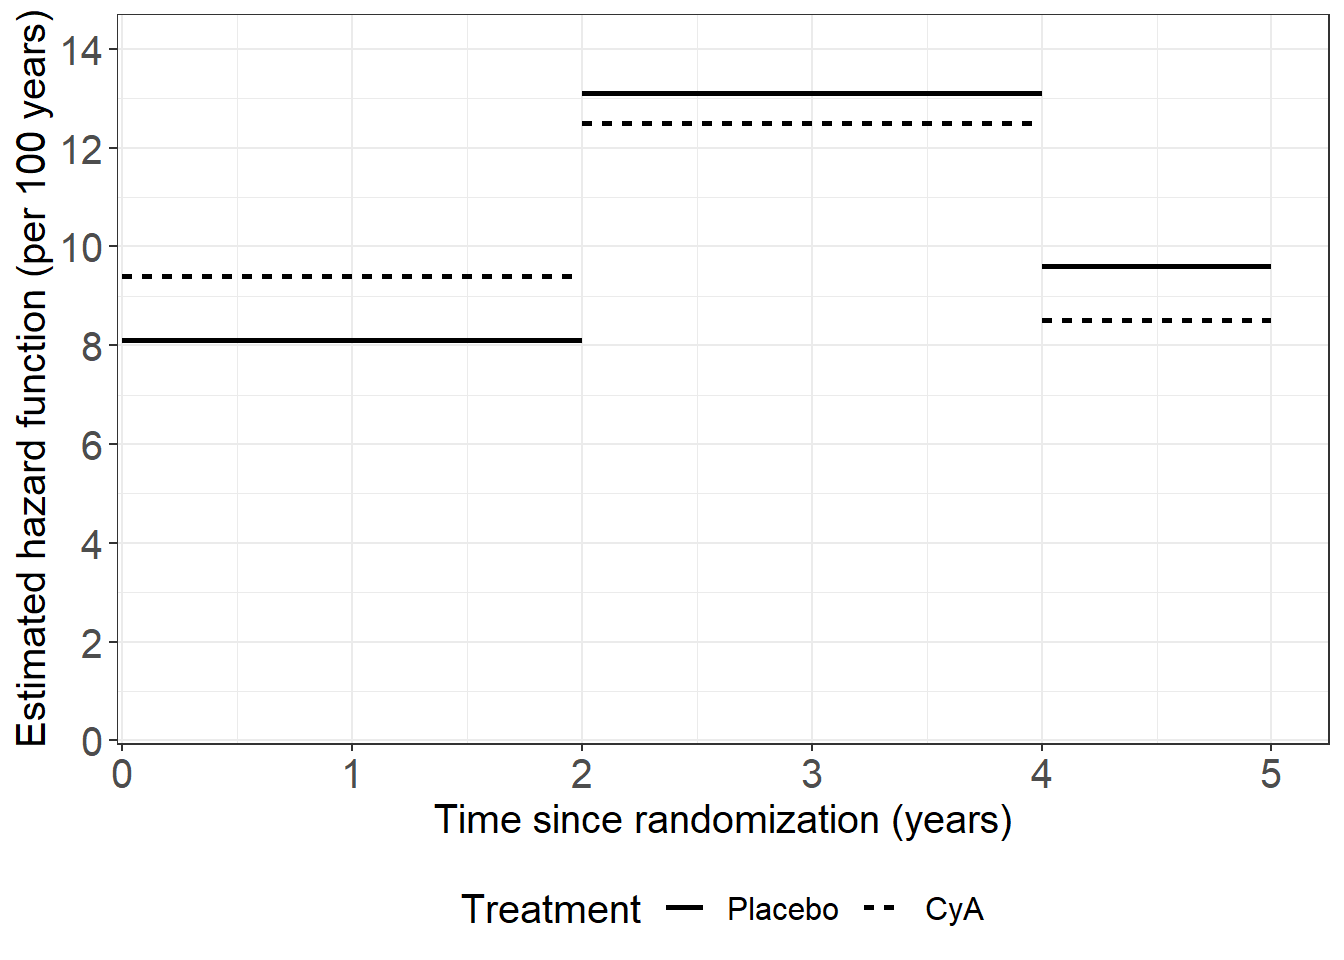
\includegraphics{./Ch2_files/figure-pdf/unnamed-chunk-3-1.pdf}

}

\end{figure}

\hypertarget{cox-models}{%
\section*{Cox model}\label{cox-models}}
\addcontentsline{toc}{section}{Cox model}

\markright{Cox model}

\begin{Shaded}
\begin{Highlighting}[]
\NormalTok{libname h }\StringTok{"data"}\NormalTok{;}
\NormalTok{data pbc3;}
\NormalTok{  set h.pbc3;}
\NormalTok{  event}\OtherTok{=}\NormalTok{status ne }\DecValTok{0}\NormalTok{; }\SpecialCharTok{*}\NormalTok{ Binary variable }\ControlFlowTok{for}\NormalTok{ events }\ControlFlowTok{for}\NormalTok{ later use;}
\NormalTok{run;}
\NormalTok{proc phreg data}\OtherTok{=}\NormalTok{pbc3;}
\NormalTok{  class }\FunctionTok{tment}\NormalTok{(}\AttributeTok{ref=}\StringTok{"0"}\NormalTok{) }\SpecialCharTok{/}\NormalTok{ param}\OtherTok{=}\NormalTok{ref ;}
\NormalTok{  model years}\SpecialCharTok{*}\FunctionTok{status}\NormalTok{(}\DecValTok{0}\NormalTok{)}\OtherTok{=}\NormalTok{tment  ;}
\NormalTok{run;}
\end{Highlighting}
\end{Shaded}

\begin{verbatim}
                                      The PHREG Procedure

                                       Model Information

                               Data Set                 WORK.PBC3
                               Dependent Variable       years    
                               Censoring Variable       status   
                               Censoring Value(s)       0        
                               Ties Handling            BRESLOW  

                            Number of Observations Read         349
                            Number of Observations Used         349

                                    Class Level Information
 
                                                       Design
                                 Class     Value     Variables

                                 tment     0                 0
                                           1                 1

                       Summary of the Number of Event and Censored Values
 
                                                               Percent
                             Total       Event    Censored    Censored

                               349          90         259       74.21

                                       Convergence Status

                         Convergence criterion (GCONV=1E-8) satisfied.          

                                     Model Fit Statistics
 
                                             Without           With
                            Criterion     Covariates     Covariates

                            -2 LOG L         948.259        948.182
                            AIC              948.259        950.182
                            SBC              948.259        952.682

                            Testing Global Null Hypothesis: BETA=0
 
                    Test                 Chi-Square       DF     Pr > ChiSq

                    Likelihood Ratio         0.0771        1         0.7813
                    Score                    0.0771        1         0.7813
                    Wald                     0.0770        1         0.7814

                                          Type 3 Tests
 
                                                   Wald
                           Effect      DF    Chi-Square    Pr > ChiSq

                           tment        1        0.0770        0.7814

                            Analysis of Maximum Likelihood Estimates
 
                      Parameter      Standard                                  Hazard
Parameter      DF      Estimate         Error    Chi-Square    Pr > ChiSq       Ratio    Label

tment     1     1      -0.05853       0.21092        0.0770        0.7814       0.943    tment 1
\end{verbatim}

\hypertarget{exercises}{%
\section{Exercises}\label{exercises}}



\end{document}
